% Generated by Sphinx.
\def\sphinxdocclass{report}
\documentclass[letterpaper,10pt,english]{sphinxmanual}

\usepackage[utf8]{inputenc}
\ifdefined\DeclareUnicodeCharacter
  \DeclareUnicodeCharacter{00A0}{\nobreakspace}
\else\fi
\usepackage{cmap}
\usepackage[T1]{fontenc}
\usepackage{amsmath,amssymb}
\usepackage{babel}
\usepackage{times}
\usepackage[Bjarne]{fncychap}
\usepackage{longtable}
\usepackage{sphinx}
\usepackage{multirow}
\usepackage{eqparbox}


\addto\captionsenglish{\renewcommand{\figurename}{Fig. }}
\addto\captionsenglish{\renewcommand{\tablename}{Table }}
\SetupFloatingEnvironment{literal-block}{name=Listing }

\addto\extrasenglish{\def\pageautorefname{page}}

\setcounter{tocdepth}{0}


\title{Enhanced Sampling Toolkit Documentation}
\date{Jul 27, 2016}
\release{0.1a}
\author{Jeremy O. B. Tempkin}
\newcommand{\sphinxlogo}{}
\renewcommand{\releasename}{Release}
\makeindex

\makeatletter
\def\PYG@reset{\let\PYG@it=\relax \let\PYG@bf=\relax%
    \let\PYG@ul=\relax \let\PYG@tc=\relax%
    \let\PYG@bc=\relax \let\PYG@ff=\relax}
\def\PYG@tok#1{\csname PYG@tok@#1\endcsname}
\def\PYG@toks#1+{\ifx\relax#1\empty\else%
    \PYG@tok{#1}\expandafter\PYG@toks\fi}
\def\PYG@do#1{\PYG@bc{\PYG@tc{\PYG@ul{%
    \PYG@it{\PYG@bf{\PYG@ff{#1}}}}}}}
\def\PYG#1#2{\PYG@reset\PYG@toks#1+\relax+\PYG@do{#2}}

\expandafter\def\csname PYG@tok@gd\endcsname{\def\PYG@tc##1{\textcolor[rgb]{0.63,0.00,0.00}{##1}}}
\expandafter\def\csname PYG@tok@gu\endcsname{\let\PYG@bf=\textbf\def\PYG@tc##1{\textcolor[rgb]{0.50,0.00,0.50}{##1}}}
\expandafter\def\csname PYG@tok@gt\endcsname{\def\PYG@tc##1{\textcolor[rgb]{0.00,0.27,0.87}{##1}}}
\expandafter\def\csname PYG@tok@gs\endcsname{\let\PYG@bf=\textbf}
\expandafter\def\csname PYG@tok@gr\endcsname{\def\PYG@tc##1{\textcolor[rgb]{1.00,0.00,0.00}{##1}}}
\expandafter\def\csname PYG@tok@cm\endcsname{\let\PYG@it=\textit\def\PYG@tc##1{\textcolor[rgb]{0.25,0.50,0.56}{##1}}}
\expandafter\def\csname PYG@tok@vg\endcsname{\def\PYG@tc##1{\textcolor[rgb]{0.73,0.38,0.84}{##1}}}
\expandafter\def\csname PYG@tok@vi\endcsname{\def\PYG@tc##1{\textcolor[rgb]{0.73,0.38,0.84}{##1}}}
\expandafter\def\csname PYG@tok@mh\endcsname{\def\PYG@tc##1{\textcolor[rgb]{0.13,0.50,0.31}{##1}}}
\expandafter\def\csname PYG@tok@cs\endcsname{\def\PYG@tc##1{\textcolor[rgb]{0.25,0.50,0.56}{##1}}\def\PYG@bc##1{\setlength{\fboxsep}{0pt}\colorbox[rgb]{1.00,0.94,0.94}{\strut ##1}}}
\expandafter\def\csname PYG@tok@ge\endcsname{\let\PYG@it=\textit}
\expandafter\def\csname PYG@tok@vc\endcsname{\def\PYG@tc##1{\textcolor[rgb]{0.73,0.38,0.84}{##1}}}
\expandafter\def\csname PYG@tok@il\endcsname{\def\PYG@tc##1{\textcolor[rgb]{0.13,0.50,0.31}{##1}}}
\expandafter\def\csname PYG@tok@go\endcsname{\def\PYG@tc##1{\textcolor[rgb]{0.20,0.20,0.20}{##1}}}
\expandafter\def\csname PYG@tok@cp\endcsname{\def\PYG@tc##1{\textcolor[rgb]{0.00,0.44,0.13}{##1}}}
\expandafter\def\csname PYG@tok@gi\endcsname{\def\PYG@tc##1{\textcolor[rgb]{0.00,0.63,0.00}{##1}}}
\expandafter\def\csname PYG@tok@gh\endcsname{\let\PYG@bf=\textbf\def\PYG@tc##1{\textcolor[rgb]{0.00,0.00,0.50}{##1}}}
\expandafter\def\csname PYG@tok@ni\endcsname{\let\PYG@bf=\textbf\def\PYG@tc##1{\textcolor[rgb]{0.84,0.33,0.22}{##1}}}
\expandafter\def\csname PYG@tok@nl\endcsname{\let\PYG@bf=\textbf\def\PYG@tc##1{\textcolor[rgb]{0.00,0.13,0.44}{##1}}}
\expandafter\def\csname PYG@tok@nn\endcsname{\let\PYG@bf=\textbf\def\PYG@tc##1{\textcolor[rgb]{0.05,0.52,0.71}{##1}}}
\expandafter\def\csname PYG@tok@no\endcsname{\def\PYG@tc##1{\textcolor[rgb]{0.38,0.68,0.84}{##1}}}
\expandafter\def\csname PYG@tok@na\endcsname{\def\PYG@tc##1{\textcolor[rgb]{0.25,0.44,0.63}{##1}}}
\expandafter\def\csname PYG@tok@nb\endcsname{\def\PYG@tc##1{\textcolor[rgb]{0.00,0.44,0.13}{##1}}}
\expandafter\def\csname PYG@tok@nc\endcsname{\let\PYG@bf=\textbf\def\PYG@tc##1{\textcolor[rgb]{0.05,0.52,0.71}{##1}}}
\expandafter\def\csname PYG@tok@nd\endcsname{\let\PYG@bf=\textbf\def\PYG@tc##1{\textcolor[rgb]{0.33,0.33,0.33}{##1}}}
\expandafter\def\csname PYG@tok@ne\endcsname{\def\PYG@tc##1{\textcolor[rgb]{0.00,0.44,0.13}{##1}}}
\expandafter\def\csname PYG@tok@nf\endcsname{\def\PYG@tc##1{\textcolor[rgb]{0.02,0.16,0.49}{##1}}}
\expandafter\def\csname PYG@tok@si\endcsname{\let\PYG@it=\textit\def\PYG@tc##1{\textcolor[rgb]{0.44,0.63,0.82}{##1}}}
\expandafter\def\csname PYG@tok@s2\endcsname{\def\PYG@tc##1{\textcolor[rgb]{0.25,0.44,0.63}{##1}}}
\expandafter\def\csname PYG@tok@nt\endcsname{\let\PYG@bf=\textbf\def\PYG@tc##1{\textcolor[rgb]{0.02,0.16,0.45}{##1}}}
\expandafter\def\csname PYG@tok@nv\endcsname{\def\PYG@tc##1{\textcolor[rgb]{0.73,0.38,0.84}{##1}}}
\expandafter\def\csname PYG@tok@s1\endcsname{\def\PYG@tc##1{\textcolor[rgb]{0.25,0.44,0.63}{##1}}}
\expandafter\def\csname PYG@tok@ch\endcsname{\let\PYG@it=\textit\def\PYG@tc##1{\textcolor[rgb]{0.25,0.50,0.56}{##1}}}
\expandafter\def\csname PYG@tok@m\endcsname{\def\PYG@tc##1{\textcolor[rgb]{0.13,0.50,0.31}{##1}}}
\expandafter\def\csname PYG@tok@gp\endcsname{\let\PYG@bf=\textbf\def\PYG@tc##1{\textcolor[rgb]{0.78,0.36,0.04}{##1}}}
\expandafter\def\csname PYG@tok@sh\endcsname{\def\PYG@tc##1{\textcolor[rgb]{0.25,0.44,0.63}{##1}}}
\expandafter\def\csname PYG@tok@ow\endcsname{\let\PYG@bf=\textbf\def\PYG@tc##1{\textcolor[rgb]{0.00,0.44,0.13}{##1}}}
\expandafter\def\csname PYG@tok@sx\endcsname{\def\PYG@tc##1{\textcolor[rgb]{0.78,0.36,0.04}{##1}}}
\expandafter\def\csname PYG@tok@bp\endcsname{\def\PYG@tc##1{\textcolor[rgb]{0.00,0.44,0.13}{##1}}}
\expandafter\def\csname PYG@tok@c1\endcsname{\let\PYG@it=\textit\def\PYG@tc##1{\textcolor[rgb]{0.25,0.50,0.56}{##1}}}
\expandafter\def\csname PYG@tok@o\endcsname{\def\PYG@tc##1{\textcolor[rgb]{0.40,0.40,0.40}{##1}}}
\expandafter\def\csname PYG@tok@kc\endcsname{\let\PYG@bf=\textbf\def\PYG@tc##1{\textcolor[rgb]{0.00,0.44,0.13}{##1}}}
\expandafter\def\csname PYG@tok@c\endcsname{\let\PYG@it=\textit\def\PYG@tc##1{\textcolor[rgb]{0.25,0.50,0.56}{##1}}}
\expandafter\def\csname PYG@tok@mf\endcsname{\def\PYG@tc##1{\textcolor[rgb]{0.13,0.50,0.31}{##1}}}
\expandafter\def\csname PYG@tok@err\endcsname{\def\PYG@bc##1{\setlength{\fboxsep}{0pt}\fcolorbox[rgb]{1.00,0.00,0.00}{1,1,1}{\strut ##1}}}
\expandafter\def\csname PYG@tok@mb\endcsname{\def\PYG@tc##1{\textcolor[rgb]{0.13,0.50,0.31}{##1}}}
\expandafter\def\csname PYG@tok@ss\endcsname{\def\PYG@tc##1{\textcolor[rgb]{0.32,0.47,0.09}{##1}}}
\expandafter\def\csname PYG@tok@sr\endcsname{\def\PYG@tc##1{\textcolor[rgb]{0.14,0.33,0.53}{##1}}}
\expandafter\def\csname PYG@tok@mo\endcsname{\def\PYG@tc##1{\textcolor[rgb]{0.13,0.50,0.31}{##1}}}
\expandafter\def\csname PYG@tok@kd\endcsname{\let\PYG@bf=\textbf\def\PYG@tc##1{\textcolor[rgb]{0.00,0.44,0.13}{##1}}}
\expandafter\def\csname PYG@tok@mi\endcsname{\def\PYG@tc##1{\textcolor[rgb]{0.13,0.50,0.31}{##1}}}
\expandafter\def\csname PYG@tok@kn\endcsname{\let\PYG@bf=\textbf\def\PYG@tc##1{\textcolor[rgb]{0.00,0.44,0.13}{##1}}}
\expandafter\def\csname PYG@tok@cpf\endcsname{\let\PYG@it=\textit\def\PYG@tc##1{\textcolor[rgb]{0.25,0.50,0.56}{##1}}}
\expandafter\def\csname PYG@tok@kr\endcsname{\let\PYG@bf=\textbf\def\PYG@tc##1{\textcolor[rgb]{0.00,0.44,0.13}{##1}}}
\expandafter\def\csname PYG@tok@s\endcsname{\def\PYG@tc##1{\textcolor[rgb]{0.25,0.44,0.63}{##1}}}
\expandafter\def\csname PYG@tok@kp\endcsname{\def\PYG@tc##1{\textcolor[rgb]{0.00,0.44,0.13}{##1}}}
\expandafter\def\csname PYG@tok@w\endcsname{\def\PYG@tc##1{\textcolor[rgb]{0.73,0.73,0.73}{##1}}}
\expandafter\def\csname PYG@tok@kt\endcsname{\def\PYG@tc##1{\textcolor[rgb]{0.56,0.13,0.00}{##1}}}
\expandafter\def\csname PYG@tok@sc\endcsname{\def\PYG@tc##1{\textcolor[rgb]{0.25,0.44,0.63}{##1}}}
\expandafter\def\csname PYG@tok@sb\endcsname{\def\PYG@tc##1{\textcolor[rgb]{0.25,0.44,0.63}{##1}}}
\expandafter\def\csname PYG@tok@k\endcsname{\let\PYG@bf=\textbf\def\PYG@tc##1{\textcolor[rgb]{0.00,0.44,0.13}{##1}}}
\expandafter\def\csname PYG@tok@se\endcsname{\let\PYG@bf=\textbf\def\PYG@tc##1{\textcolor[rgb]{0.25,0.44,0.63}{##1}}}
\expandafter\def\csname PYG@tok@sd\endcsname{\let\PYG@it=\textit\def\PYG@tc##1{\textcolor[rgb]{0.25,0.44,0.63}{##1}}}

\def\PYGZbs{\char`\\}
\def\PYGZus{\char`\_}
\def\PYGZob{\char`\{}
\def\PYGZcb{\char`\}}
\def\PYGZca{\char`\^}
\def\PYGZam{\char`\&}
\def\PYGZlt{\char`\<}
\def\PYGZgt{\char`\>}
\def\PYGZsh{\char`\#}
\def\PYGZpc{\char`\%}
\def\PYGZdl{\char`\$}
\def\PYGZhy{\char`\-}
\def\PYGZsq{\char`\'}
\def\PYGZdq{\char`\"}
\def\PYGZti{\char`\~}
% for compatibility with earlier versions
\def\PYGZat{@}
\def\PYGZlb{[}
\def\PYGZrb{]}
\makeatother

\renewcommand\PYGZsq{\textquotesingle}

\begin{document}

\maketitle
\tableofcontents
\phantomsection\label{index::doc}



\chapter{Introduction}
\label{introduction.doc:introduction}\label{introduction.doc:welcome-to-enhanced-sampling-toolkit-s-documentation}\label{introduction.doc::doc}
The objective of the Enhanced Sampling Toolkit is to provide a set of tools that facilitates rapid prototyping and development of enhanced sampling algorithms in Python.

The toolkit is implemented in 100\% Python. One reason for this decision is that Python is a popular language in the broader scientific community and has a wide support base for developing scientific codes. However, more importantly, a strength of the language lies in the speed at which ideas can be implemented into working code. Since rapid and flexible prototyping of new algorithms is the core priority of the toolkit, Python seems a natural choice in language. However, if the need arises in a future date, ports to other languages may be considered and integrated into the package.

In many places of the toolkit some care has been made to adhere to the powerful Python object design principles inherent in the Python data model. We find this to be a powerful feature of the Python language since it facilitates clean, ``Pythonic'' use of the toolkit in our applications. We are continually working to improve this aspect of the toolkit as the project develops.

In addition to rapid algorithm prototyping, we've found in it's development that the toolkit is effective in HPC environments as well. Because the underlying dynamics are executed in commonly used MD codes, the toolkit has access to the HPC features that have been optimized in these codes and can therefore leverage MPI parallelism concurrently at the algorithm level and the MD level as well as support for accelerators such as GPU's or Intel MIC cards.


\section{Organization of the Toolkit}
\label{introduction.doc:organization-of-the-toolkit}
The toolkit consists of two fundamental layers. At the core of the toolkit is the Walker API. This API provides an standard interface between the algorithm level code and the code that executes the dynamical model. In the case of molecular dynamics, this API has been implemented around difference MD engines such as OpenMM or LAMMPS.

In the basic sense, the toolkit serves to wrap commonly used MD codes and in the process abstract the interactions between algorithm level code and the MD engine. This abstractions provides useful extensibilty in the sense that algorithm codes that are implemented in the Walker API can be reused and swapped between MD models and even entire MD codes. Furthermore, the expensive integration steps are executed in faster compiled codes and avoids some of the inefficiencies introduced in the choice of Python.

The second layer of the toolkit is the application tools. These set of tools provide a set of high-level modules that facilitate rapid programming of new Enhanced Sampling algorithms. These modules serve to act as reference implementations of core data structures and operations that are common to a set of enhanced sampling algorithms. In some cases, these tools rely on functionality provided by the Walker API.


\chapter{Installation}
\label{installation.doc:installation}\label{installation.doc::doc}
To install the Enhanced Sampling Toolkit on your local machine, download the package from the \href{https://github.com/jtempkin/enhanced\_sampling\_toolkit}{Github page}.

To install the toolkit, run

\begin{Verbatim}[commandchars=\\\{\}]
\PYG{n}{python} \PYG{n}{setup}\PYG{o}{.}\PYG{n}{py} \PYG{n}{install}
\end{Verbatim}

from the root of the toolkit package. If you plan on developing the files in the toolkit, use

\begin{Verbatim}[commandchars=\\\{\}]
\PYG{n}{python} \PYG{n}{setup}\PYG{o}{.}\PYG{n}{py} \PYG{n}{develop}
\end{Verbatim}

which will use the state of the local files. Note that this will allow changes made locally to the package files to visible in your Python environment.


\chapter{Walker API}
\label{walker_api/walker_api.doc::doc}\label{walker_api/walker_api.doc:walker-api}
The Walker API is built to provide an abstract interface between the ``algorithm'' level code and the code that implements the underlying dynamical model.

This section describes some of the basic usage of the implementation of the walker API for the LAMMPS package. The example pages are written from Jupyter notebooks included in the `data/' directory for interactive use. The full API is documented in the last section.


\section{LAMMPS Walker Module}
\label{walker_api/walker_api.doc:lammps-walker-module}
This module implements the Walker API for the LAMMPS MD engine. See walker\_base.py for a specification of the API. For details concerning the usage of the LAMMPS MD package see the excellent documentation at the LAMMPS webpage:

\url{http://lammps.sandia.gov/}

In particular, you may want to see how the Python wrapper to LAMMPS on which this implementation is based:

\url{http://lammps.sandia.gov/doc/Section\_python.html}

To use the LAMMPS walker module provided in the toolkit, you will need to have the LAMMPS MD engine available as an importable Python module. Please follow in the instructions provided by the above link to download, compile and install LAMMPS for Python. To check to see if LAMMPS is installed correctly, try importing it interactively as

\begin{Verbatim}[commandchars=\\\{\}]
\PYG{k+kn}{from} \PYG{n+nn}{lammps} \PYG{k}{import} \PYG{n}{lammps}
\end{Verbatim}

If this import returns no errors, the LAMMPS Walker module should be able to import and use the compiled LAMMPS build on your machine.


\section{LAMMPS Walker Basic Usage}
\label{walker_api/walker_api.doc:lammps-walker-basic-usage}
In this notebook, we will highlight some examples of how the LAMMPS
Walker API implementation can be used.

\begin{Verbatim}[commandchars=\\\{\}]
\PYG{o}{\PYGZpc{}}\PYG{n}{matplotlib} \PYG{n}{inline}
\PYG{k+kn}{from} \PYG{n+nn}{matplotlib} \PYG{k}{import} \PYG{n}{pyplot} \PYG{k}{as} \PYG{n}{plt}

\PYG{c+c1}{\PYGZsh{} import the LAMMPS walker binding}
\PYG{k+kn}{from} \PYG{n+nn}{walker\PYGZus{}api} \PYG{k}{import} \PYG{n}{lammps\PYGZus{}walker}

\PYG{c+c1}{\PYGZsh{} instantiate a copy using the example input script}
\PYG{n}{walker} \PYG{o}{=} \PYG{n}{lammps\PYGZus{}walker}\PYG{o}{.}\PYG{n}{Lammps}\PYG{p}{(}\PYG{l+s+s2}{\PYGZdq{}}\PYG{l+s+s2}{input.diala}\PYG{l+s+s2}{\PYGZdq{}}\PYG{p}{,} \PYG{k+kc}{None}\PYG{p}{)}
\end{Verbatim}

The underlying model for the alanine dipeptide in vacuum is specificed
in the ``input.diala'' file. This input file is read by LAMMPS's own
command parser, so it should be written as a standard LAMMPS input file.

You can use the API routines to interrogate certain properties of the
model, such as returning an array of the positions currently stored, or
the coordinates of some collective variables which are implemented as
LAMMPS computes.

The following script generates a time-series of the phi dihedral angle
for the alanine dipeptide in vacuum.

\begin{Verbatim}[commandchars=\\\{\}]
\PYG{c+c1}{\PYGZsh{} get an array of the initial position}
\PYG{n}{initial\PYGZus{}position} \PYG{o}{=} \PYG{n}{walker}\PYG{o}{.}\PYG{n}{get\PYGZus{}position}\PYG{p}{(}\PYG{p}{)}
\PYG{n}{initial\PYGZus{}time} \PYG{o}{=} \PYG{n}{walker}\PYG{o}{.}\PYG{n}{get\PYGZus{}time}\PYG{p}{(}\PYG{p}{)}

\PYG{c+c1}{\PYGZsh{} remove any set walker collective variables}
\PYG{n}{walker}\PYG{o}{.}\PYG{n}{destroy\PYGZus{}colvars}\PYG{p}{(}\PYG{p}{)}

\PYG{c+c1}{\PYGZsh{} add the phi dihedral with name \PYGZdq{}phi\PYGZdq{}}
\PYG{n}{walker}\PYG{o}{.}\PYG{n}{add\PYGZus{}colvars}\PYG{p}{(}\PYG{l+s+s2}{\PYGZdq{}}\PYG{l+s+s2}{phi}\PYG{l+s+s2}{\PYGZdq{}}\PYG{p}{,} \PYG{l+s+s2}{\PYGZdq{}}\PYG{l+s+s2}{dihedral}\PYG{l+s+s2}{\PYGZdq{}}\PYG{p}{,} \PYG{p}{[}\PYG{l+m+mi}{5}\PYG{p}{,}\PYG{l+m+mi}{7}\PYG{p}{,}\PYG{l+m+mi}{9}\PYG{p}{,}\PYG{l+m+mi}{15}\PYG{p}{]}\PYG{p}{)}

\PYG{n}{colvars} \PYG{o}{=} \PYG{p}{[}\PYG{p}{]}

\PYG{c+c1}{\PYGZsh{} now we\PYGZsq{}ll sample the phi dihedral}
\PYG{k}{for} \PYG{n}{i} \PYG{o+ow}{in} \PYG{n+nb}{range}\PYG{p}{(}\PYG{l+m+mi}{1000}\PYG{p}{)}\PYG{p}{:}

    \PYG{c+c1}{\PYGZsh{} move the walker forward in time}
    \PYG{n}{walker}\PYG{o}{.}\PYG{n}{propagate}\PYG{p}{(}\PYG{l+m+mi}{1000}\PYG{p}{)}

    \PYG{c+c1}{\PYGZsh{} record the value of the phi dihedral}
    \PYG{n}{cv} \PYG{o}{=} \PYG{n}{walker}\PYG{o}{.}\PYG{n}{get\PYGZus{}colvars}\PYG{p}{(}\PYG{p}{)}
    \PYG{n}{colvars}\PYG{o}{.}\PYG{n}{append}\PYG{p}{(}\PYG{n}{cv}\PYG{p}{)}


\PYG{c+c1}{\PYGZsh{} plot the timeseries}
\PYG{n}{plt}\PYG{o}{.}\PYG{n}{plot}\PYG{p}{(}\PYG{n}{colvars}\PYG{p}{)}
\PYG{n}{plt}\PYG{o}{.}\PYG{n}{xlabel}\PYG{p}{(}\PYG{l+s+s2}{\PYGZdq{}}\PYG{l+s+s2}{time (ps)}\PYG{l+s+s2}{\PYGZdq{}}\PYG{p}{)}
\PYG{n}{plt}\PYG{o}{.}\PYG{n}{ylabel}\PYG{p}{(}\PYG{l+s+s2}{\PYGZdq{}}\PYG{l+s+s2}{phi (degrees)}\PYG{l+s+s2}{\PYGZdq{}}\PYG{p}{)}
\PYG{n}{plt}\PYG{o}{.}\PYG{n}{ylim}\PYG{p}{(}\PYG{p}{[}\PYG{o}{\PYGZhy{}}\PYG{l+m+mi}{180}\PYG{p}{,} \PYG{l+m+mi}{180}\PYG{p}{]}\PYG{p}{)}
\end{Verbatim}

\begin{Verbatim}[commandchars=\\\{\}]
\PYG{p}{(}\PYG{o}{\PYGZhy{}}\PYG{l+m+mi}{180}\PYG{p}{,} \PYG{l+m+mi}{180}\PYG{p}{)}
\end{Verbatim}

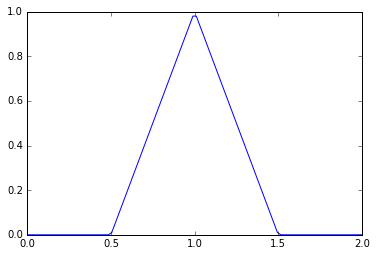
\includegraphics{{walker_api/output_3_1}.png}

\begin{Verbatim}[commandchars=\\\{\}]
\PYG{c+c1}{\PYGZsh{} we can set and reset the}
\end{Verbatim}

Please see the included iPython notebook for an interactive version of
this embedded code.


\section{LAMMPS Walker API}
\label{walker_api/walker_api.doc:lammps-walker-api}\label{walker_api/walker_api.doc:module-walker_api.lammps_walker}\index{walker\_api.lammps\_walker (module)}
This class implements the enhanced sampling walker API for the bindings to the
LAMMPS package.
\index{Lammps (class in walker\_api.lammps\_walker)}

\begin{fulllineitems}
\phantomsection\label{walker_api/walker_api.doc:walker_api.lammps_walker.Lammps}\pysiglinewithargsret{\strong{class }\code{walker\_api.lammps\_walker.}\bfcode{Lammps}}{\emph{inputFilename}, \emph{logFilename}, \emph{index=0}, \emph{debug=False}}{}
Implements the Walker API using the LAMMPS engine.
\index{add\_colvars() (walker\_api.lammps\_walker.Lammps method)}

\begin{fulllineitems}
\phantomsection\label{walker_api/walker_api.doc:walker_api.lammps_walker.Lammps.add_colvars}\pysiglinewithargsret{\bfcode{add\_colvars}}{\emph{name}, \emph{cvType}, \emph{atomIDs}}{}
Add a collective variable to the walker.

The following variables are currently supported:
\begin{itemize}
\item {} 
`bond'

\item {} 
`angle'

\item {} 
`dihedral'

\item {} 
`x', `y', `z' position components

\item {} 
`x', `y', `z' velocity components

\end{itemize}

The atomIDs must list the atoms indecies involved and should provide the right number of atom indecies for the collective variable:
\begin{itemize}
\item {} 
`bond' -\textgreater{} 2

\item {} 
`angle'-\textgreater{} 3

\item {} 
`dihedral' -\textgreater{} 4

\item {} 
position or velocity component -\textgreater{} 1

\end{itemize}

Note that due to feature of LAMMPS's implementation, the bond, angle or dihedral must be know in the topology of the LAMMPS data file. I.e. LAMMPS must be able to build this compute without an error.
\begin{quote}\begin{description}
\item[{Parameters}] \leavevmode
\textbf{name} : string
\begin{quote}

A string used to reference this collective variable. Collective variable names must be unique.
\end{quote}

\textbf{cvType} : string
\begin{quote}

A string refering to the type of collective variable.
\end{quote}

\textbf{atomIDs} : list
\begin{quote}

A list of the atom indecies involved in the collective variable.
\end{quote}

\end{description}\end{quote}

\end{fulllineitems}

\index{close() (walker\_api.lammps\_walker.Lammps method)}

\begin{fulllineitems}
\phantomsection\label{walker_api/walker_api.doc:walker_api.lammps_walker.Lammps.close}\pysiglinewithargsret{\bfcode{close}}{}{}
Close the underlying LAMMPS object.

\end{fulllineitems}

\index{command() (walker\_api.lammps\_walker.Lammps method)}

\begin{fulllineitems}
\phantomsection\label{walker_api/walker_api.doc:walker_api.lammps_walker.Lammps.command}\pysiglinewithargsret{\bfcode{command}}{\emph{command}}{}
Issue a LAMMPS command directly to the LAMMPS code.
\begin{quote}\begin{description}
\item[{Parameters}] \leavevmode
\textbf{command} : string
\begin{quote}

A command to pass directy to LAMMPS's command interpreter.
\end{quote}

\end{description}\end{quote}

\end{fulllineitems}

\index{destroy\_colvars() (walker\_api.lammps\_walker.Lammps method)}

\begin{fulllineitems}
\phantomsection\label{walker_api/walker_api.doc:walker_api.lammps_walker.Lammps.destroy_colvars}\pysiglinewithargsret{\bfcode{destroy\_colvars}}{}{}
Remove all collective variables from the walker instance.

\end{fulllineitems}

\index{draw\_velocity() (walker\_api.lammps\_walker.Lammps method)}

\begin{fulllineitems}
\phantomsection\label{walker_api/walker_api.doc:walker_api.lammps_walker.Lammps.draw_velocity}\pysiglinewithargsret{\bfcode{draw\_velocity}}{\emph{distType='gaussian'}, \emph{temperature=310.0}, \emph{seed=None}}{}
Redraw the velocity of the walker.

Current supports the following distributions:
\begin{itemize}
\item {} 
`gaussian'

\end{itemize}

\end{fulllineitems}

\index{equilibrate() (walker\_api.lammps\_walker.Lammps method)}

\begin{fulllineitems}
\phantomsection\label{walker_api/walker_api.doc:walker_api.lammps_walker.Lammps.equilibrate}\pysiglinewithargsret{\bfcode{equilibrate}}{\emph{center}, \emph{restraint}, \emph{numSteps}}{}
Equilibrate the walker to a value of the collective variabales.

This equilibrates the system to the target value in the collective variable space. It applies a harmonic restraint at the specified coordinates with a given strength and runs a fixed number of dynamics steps. Note that sequences of the equilibrate commands can be used to implement dragging protocols.

The length of the center and restraint parameters must match the length of the length of the collective variable array.
\begin{quote}\begin{description}
\item[{Parameters}] \leavevmode
\textbf{center} : list
\begin{quote}

A list of the centers of the harmonic restraint in collective variables space.
\end{quote}

\textbf{restraint} : list
\begin{quote}

A list of the strength of the harmonic.
\end{quote}

\textbf{numSteps} : int
\begin{quote}

Number of dynamics timesteps to integrate.
\end{quote}

\end{description}\end{quote}

\end{fulllineitems}

\index{get\_colvars() (walker\_api.lammps\_walker.Lammps method)}

\begin{fulllineitems}
\phantomsection\label{walker_api/walker_api.doc:walker_api.lammps_walker.Lammps.get_colvars}\pysiglinewithargsret{\bfcode{get\_colvars}}{}{}
Return the values of the collective variables.
\begin{quote}\begin{description}
\item[{Returns}] \leavevmode
numpy.ndarray
\begin{quote}

A numpy array of the collective variables computed by this walker
\end{quote}

\end{description}\end{quote}

\end{fulllineitems}

\index{get\_position() (walker\_api.lammps\_walker.Lammps method)}

\begin{fulllineitems}
\phantomsection\label{walker_api/walker_api.doc:walker_api.lammps_walker.Lammps.get_position}\pysiglinewithargsret{\bfcode{get\_position}}{}{}
Return the spatial coordinates of the walker.
\begin{quote}\begin{description}
\item[{Returns}] \leavevmode
numpy.ndarray
\begin{quote}

A one-dimensional array of the coordinates in {[}x1, y1, z1, x2, y2, z2,...{]} format.
\end{quote}

\end{description}\end{quote}

\end{fulllineitems}

\index{get\_time() (walker\_api.lammps\_walker.Lammps method)}

\begin{fulllineitems}
\phantomsection\label{walker_api/walker_api.doc:walker_api.lammps_walker.Lammps.get_time}\pysiglinewithargsret{\bfcode{get\_time}}{}{}
Return the current time in number of timesteps.
\begin{quote}\begin{description}
\item[{Returns}] \leavevmode
\textbf{time} : integer
\begin{quote}

Returns the number of model time steps taken.
\end{quote}

\end{description}\end{quote}

\end{fulllineitems}

\index{get\_velocity() (walker\_api.lammps\_walker.Lammps method)}

\begin{fulllineitems}
\phantomsection\label{walker_api/walker_api.doc:walker_api.lammps_walker.Lammps.get_velocity}\pysiglinewithargsret{\bfcode{get\_velocity}}{}{}
Return the velocity of the walker.
\begin{quote}\begin{description}
\item[{Returns}] \leavevmode
numpy.ndarray
\begin{quote}

A one dimensional array of the velocities in {[}vx1, vy1, vz1, vx2, vy2, vz2,...{]} format.
\end{quote}

\end{description}\end{quote}

\end{fulllineitems}

\index{minimize() (walker\_api.lammps\_walker.Lammps method)}

\begin{fulllineitems}
\phantomsection\label{walker_api/walker_api.doc:walker_api.lammps_walker.Lammps.minimize}\pysiglinewithargsret{\bfcode{minimize}}{\emph{args=None}}{}
Perform a steepest descent minimization.

\end{fulllineitems}

\index{propagate() (walker\_api.lammps\_walker.Lammps method)}

\begin{fulllineitems}
\phantomsection\label{walker_api/walker_api.doc:walker_api.lammps_walker.Lammps.propagate}\pysiglinewithargsret{\bfcode{propagate}}{\emph{numSteps}, \emph{pre='no'}, \emph{post='no'}}{}
Integrate the dynamics forward in time.

This routine integrates the dynamics of the underlying model. It expects an integer number specifying the number of time steps to take.
\begin{quote}\begin{description}
\item[{Parameters}] \leavevmode
\textbf{numSteps} : int
\begin{quote}

The number of model timesteps to take.
\end{quote}

\textbf{pre} : string (`no')
\begin{quote}

Run the pre-dynamics setup in LAMMPS if set to `yes'.
\end{quote}

\textbf{post} : string (`no')
\begin{quote}

Run the post-dynamics timings in LAMMPS if set to `yes'.
\end{quote}

\end{description}\end{quote}

\end{fulllineitems}

\index{remove\_output() (walker\_api.lammps\_walker.Lammps method)}

\begin{fulllineitems}
\phantomsection\label{walker_api/walker_api.doc:walker_api.lammps_walker.Lammps.remove_output}\pysiglinewithargsret{\bfcode{remove\_output}}{}{}
Remove all output for the model.

\end{fulllineitems}

\index{reverse\_velocity() (walker\_api.lammps\_walker.Lammps method)}

\begin{fulllineitems}
\phantomsection\label{walker_api/walker_api.doc:walker_api.lammps_walker.Lammps.reverse_velocity}\pysiglinewithargsret{\bfcode{reverse\_velocity}}{}{}
Reverse the velocity of the walker.

This routine reverses the sign of the velocities.

\end{fulllineitems}

\index{set\_dynamics() (walker\_api.lammps\_walker.Lammps method)}

\begin{fulllineitems}
\phantomsection\label{walker_api/walker_api.doc:walker_api.lammps_walker.Lammps.set_dynamics}\pysiglinewithargsret{\bfcode{set\_dynamics}}{\emph{dynamics\_instance}}{}
Apply a dynamics model to the walker.
\begin{quote}\begin{description}
\item[{Parameters}] \leavevmode
\textbf{dynamics\_instance} : dynamics
\begin{quote}

Set up the dynamics model from the dynamics instance passed.
\end{quote}

\end{description}\end{quote}

\end{fulllineitems}

\index{set\_output() (walker\_api.lammps\_walker.Lammps method)}

\begin{fulllineitems}
\phantomsection\label{walker_api/walker_api.doc:walker_api.lammps_walker.Lammps.set_output}\pysiglinewithargsret{\bfcode{set\_output}}{\emph{name}, \emph{outputType}, \emph{filename}, \emph{nSteps}}{}
Set an output file for coordinates from the dynamics model.
\begin{quote}\begin{description}
\item[{Parameters}] \leavevmode
\textbf{name} : string
\begin{quote}

A string identifying this output type.
\end{quote}

\textbf{outputType} : string
\begin{quote}

A string identifying the output file type.
\end{quote}

\textbf{filename} : string
\begin{quote}

A string with the filename to write dynamics output.
\end{quote}

\textbf{nSteps} : int
\begin{quote}

The number of model timesteps bewteen which to write.s
\end{quote}

\end{description}\end{quote}

\end{fulllineitems}

\index{set\_position() (walker\_api.lammps\_walker.Lammps method)}

\begin{fulllineitems}
\phantomsection\label{walker_api/walker_api.doc:walker_api.lammps_walker.Lammps.set_position}\pysiglinewithargsret{\bfcode{set\_position}}{\emph{config}}{}
Set the spatial coordinates of the walker.
\begin{quote}\begin{description}
\item[{Parameters}] \leavevmode
\textbf{config} : numpy.ndarray
\begin{quote}

A one-dimentional numpy array of the position coordinates in {[}x1, y1, z1, x2, y2, z2,...{]} format.
\end{quote}

\end{description}\end{quote}

\end{fulllineitems}

\index{set\_temperature() (walker\_api.lammps\_walker.Lammps method)}

\begin{fulllineitems}
\phantomsection\label{walker_api/walker_api.doc:walker_api.lammps_walker.Lammps.set_temperature}\pysiglinewithargsret{\bfcode{set\_temperature}}{\emph{temp}}{}
Set the temperature.

This command works only if the dynamics was set with the set\_dynamics routine. Otherwise, dynamcis is set by input script provided at initialization.
\begin{quote}\begin{description}
\item[{Parameters}] \leavevmode
\textbf{temp} : float
\begin{quote}

The temperature in LAMMPS units.
\end{quote}

\end{description}\end{quote}

\end{fulllineitems}

\index{set\_time() (walker\_api.lammps\_walker.Lammps method)}

\begin{fulllineitems}
\phantomsection\label{walker_api/walker_api.doc:walker_api.lammps_walker.Lammps.set_time}\pysiglinewithargsret{\bfcode{set\_time}}{\emph{t}}{}
Set the time of the walker.

This routine expects an integer time in the number of model timesteps.
\begin{quote}\begin{description}
\item[{Parameters}] \leavevmode
\textbf{t} : integer
\begin{quote}

An integer specifying the number of model timesteps taken.
\end{quote}

\end{description}\end{quote}

\end{fulllineitems}

\index{set\_timestep() (walker\_api.lammps\_walker.Lammps method)}

\begin{fulllineitems}
\phantomsection\label{walker_api/walker_api.doc:walker_api.lammps_walker.Lammps.set_timestep}\pysiglinewithargsret{\bfcode{set\_timestep}}{\emph{timestep}}{}
Set the timestep of the integrator for the dynamics model.

This command sets the timestep used in the model's integration routine.
\begin{quote}\begin{description}
\item[{Parameters}] \leavevmode
\textbf{timestep} : float
\begin{quote}

The integration timestep.
\end{quote}

\end{description}\end{quote}

\end{fulllineitems}

\index{set\_velocity() (walker\_api.lammps\_walker.Lammps method)}

\begin{fulllineitems}
\phantomsection\label{walker_api/walker_api.doc:walker_api.lammps_walker.Lammps.set_velocity}\pysiglinewithargsret{\bfcode{set\_velocity}}{\emph{vel}}{}
Set the velocity of the walker.
\begin{quote}\begin{description}
\item[{Parameters}] \leavevmode
\textbf{vel} : numpy.ndarray
\begin{quote}

A one-dimentional array of the velocities in {[}vx1, vy1, vz1, vx2, vy2, vz2,...{]} format.
\end{quote}

\end{description}\end{quote}

\end{fulllineitems}


\end{fulllineitems}



\chapter{Nonequilibrium Umbrella Sampling (NEUS)}
\label{neus/neus.doc:nonequilibrium-umbrella-sampling-neus}\label{neus/neus.doc::doc}\label{neus/neus.doc:module-neus}\index{neus (module)}
The Nonequilibrium Umbrella Sampling (NEUS) application module provides a flexible set of tools built on top of the Walker API that implements the components of the NEUS algorithm described in (NEUS paper citation).

The NEUS toolkit provided in this package contains three modules:
\begin{itemize}
\item {} 
A module called Window that implements the data structures and routines that represent a single spatiotemporal discretization in the NEUS scheme. An instance of the Window object corresponds to a single value of the \(J^{(t)}\) process.

\item {} 
A module called partition acts as a collection of these windows objects that expresses the full \(J^{(t)}\) index space.

\item {} 
A module called entry points that provides a named tuple for storing phase space points as elements in the \(\tilde \gamma_{ij}\)

\end{itemize}

Below we describe the basic usage of the NEUS toolkit. Please see the Jupyter notebooks provided in the data folder for an interactive version.


\section{NEUS Module Basic Usage}
\label{neus/neus.doc:neus-module-basic-usage}

\subsection{NEUS Application Basic Usage Guide}
\label{neus/neus.doc:neus-application-basic-usage-guide}
The NEUS application later is composed of two fundamental objects:
\begin{itemize}
\item {} 
A Window object

\item {} 
A partition object

\end{itemize}

The Window object represents the data structures and routines that
represent a single spatiotemporal restriction, or a single ``window'' in
your NEUS scheme. In the language of NEUS, this corresponds to a single
restricted value of the \(J^{(t)}\) process.

The partition object represents a list of Window instances. Again, in
the language of NEUS, it represents the full space of the
\(J^{(t)}\) process.

In the following, we will illustrate some basic usage of these objects
with the idea of familiarizing the user with their tools and syntax. For
a fuller example of how one can use these tools to do a full NEUS
calculation, please refer to the examples section.

Ok, let's write out the goals of this section:
\begin{itemize}
\item {} 
illustrate the basic usage + syntax of the NEUS objects

\item {} 
show how these objects can be used to set up an NEUS calculation in
the language of the paper.

\end{itemize}


\subsubsection{Window objects}
\label{neus/neus.doc:window-objects}
Let's start with the windows. The NEUS application in the toolkit
provides a parent module. Different shapes of the supports in space-time
are supported by class inherentence.


\subsubsection{Partition objects}
\label{neus/neus.doc:partition-objects}
To initialize a partition object:

\begin{Verbatim}[commandchars=\\\{\}]
\PYG{k+kn}{import} \PYG{n+nn}{partition}
\PYG{k+kn}{import} \PYG{n+nn}{numpy} \PYG{k}{as} \PYG{n+nn}{np}
\PYG{n}{sys} \PYG{o}{=} \PYG{n}{partition}\PYG{o}{.}\PYG{n}{partition}\PYG{p}{(}\PYG{p}{)}
\end{Verbatim}

One can add elements to the partition one by one:

\begin{Verbatim}[commandchars=\\\{\}]
\PYG{c+c1}{\PYGZsh{} import a window object with a pyramid support}
\PYG{k+kn}{import} \PYG{n+nn}{pyramid}
\PYG{n}{win} \PYG{o}{=} \PYG{n}{pyramid}\PYG{o}{.}\PYG{n}{Pyramid}\PYG{p}{(}\PYG{p}{[}\PYG{l+m+mf}{0.0}\PYG{p}{]}\PYG{p}{,} \PYG{p}{[}\PYG{l+m+mf}{1.0}\PYG{p}{]}\PYG{p}{)}

\PYG{n}{sys}\PYG{o}{.}\PYG{n}{append}\PYG{p}{(}\PYG{n}{win}\PYG{p}{)}

\PYG{n+nb}{print} \PYG{n}{sys}
\end{Verbatim}

\begin{Verbatim}[commandchars=\\\{\}]
\PYG{n}{partition}\PYG{p}{(}\PYG{p}{[}\PYG{n}{Pyramid}\PYG{p}{(}\PYG{p}{[} \PYG{l+m+mf}{0.}\PYG{p}{]}\PYG{p}{,} \PYG{p}{[} \PYG{l+m+mf}{1.}\PYG{p}{]}\PYG{p}{)}\PYG{p}{,} \PYG{n}{Pyramid}\PYG{p}{(}\PYG{p}{[} \PYG{l+m+mf}{0.}\PYG{p}{]}\PYG{p}{,} \PYG{p}{[} \PYG{l+m+mf}{1.}\PYG{p}{]}\PYG{p}{)}\PYG{p}{,} \PYG{n}{Pyramid}\PYG{p}{(}\PYG{p}{[} \PYG{l+m+mf}{0.}\PYG{p}{]}\PYG{p}{,} \PYG{p}{[} \PYG{l+m+mf}{1.}\PYG{p}{]}\PYG{p}{)}\PYG{p}{]}\PYG{p}{)}
\end{Verbatim}

Or hand partition a list at initialization:

\begin{Verbatim}[commandchars=\\\{\}]
\PYG{n}{windows} \PYG{o}{=} \PYG{p}{[}\PYG{n}{pyramid}\PYG{o}{.}\PYG{n}{Pyramid}\PYG{p}{(}\PYG{n}{i}\PYG{p}{,}\PYG{p}{[}\PYG{l+m+mf}{1.0}\PYG{p}{]}\PYG{p}{)} \PYG{k}{for} \PYG{n}{i} \PYG{o+ow}{in} \PYG{n}{np}\PYG{o}{.}\PYG{n}{linspace}\PYG{p}{(}\PYG{l+m+mf}{0.0}\PYG{p}{,} \PYG{l+m+mf}{10.0}\PYG{p}{,} \PYG{l+m+mi}{11}\PYG{p}{)}\PYG{p}{]}
\PYG{n}{sys} \PYG{o}{=} \PYG{n}{partition}\PYG{o}{.}\PYG{n}{partition}\PYG{p}{(}\PYG{n}{windows}\PYG{p}{)}
\PYG{n+nb}{print} \PYG{n}{sys}
\end{Verbatim}

\begin{Verbatim}[commandchars=\\\{\}]
\PYG{n}{partition}\PYG{p}{(}\PYG{p}{[}\PYG{n}{Pyramid}\PYG{p}{(}\PYG{l+m+mf}{0.0}\PYG{p}{,} \PYG{p}{[} \PYG{l+m+mf}{1.}\PYG{p}{]}\PYG{p}{)}\PYG{p}{,} \PYG{n}{Pyramid}\PYG{p}{(}\PYG{l+m+mf}{1.0}\PYG{p}{,} \PYG{p}{[} \PYG{l+m+mf}{1.}\PYG{p}{]}\PYG{p}{)}\PYG{p}{,} \PYG{n}{Pyramid}\PYG{p}{(}\PYG{l+m+mf}{2.0}\PYG{p}{,} \PYG{p}{[} \PYG{l+m+mf}{1.}\PYG{p}{]}\PYG{p}{)}\PYG{p}{,} \PYG{n}{Pyramid}\PYG{p}{(}\PYG{l+m+mf}{3.0}\PYG{p}{,} \PYG{p}{[} \PYG{l+m+mf}{1.}\PYG{p}{]}\PYG{p}{)}\PYG{p}{,} \PYG{n}{Pyramid}\PYG{p}{(}\PYG{l+m+mf}{4.0}\PYG{p}{,} \PYG{p}{[} \PYG{l+m+mf}{1.}\PYG{p}{]}\PYG{p}{)}\PYG{p}{,} \PYG{n}{Pyramid}\PYG{p}{(}\PYG{l+m+mf}{5.0}\PYG{p}{,} \PYG{p}{[} \PYG{l+m+mf}{1.}\PYG{p}{]}\PYG{p}{)}\PYG{p}{,} \PYG{n}{Pyramid}\PYG{p}{(}\PYG{l+m+mf}{6.0}\PYG{p}{,} \PYG{p}{[} \PYG{l+m+mf}{1.}\PYG{p}{]}\PYG{p}{)}\PYG{p}{,} \PYG{n}{Pyramid}\PYG{p}{(}\PYG{l+m+mf}{7.0}\PYG{p}{,} \PYG{p}{[} \PYG{l+m+mf}{1.}\PYG{p}{]}\PYG{p}{)}\PYG{p}{,} \PYG{n}{Pyramid}\PYG{p}{(}\PYG{l+m+mf}{8.0}\PYG{p}{,} \PYG{p}{[} \PYG{l+m+mf}{1.}\PYG{p}{]}\PYG{p}{)}\PYG{p}{,} \PYG{n}{Pyramid}\PYG{p}{(}\PYG{l+m+mf}{9.0}\PYG{p}{,} \PYG{p}{[} \PYG{l+m+mf}{1.}\PYG{p}{]}\PYG{p}{)}\PYG{p}{,} \PYG{n}{Pyramid}\PYG{p}{(}\PYG{l+m+mf}{10.0}\PYG{p}{,} \PYG{p}{[} \PYG{l+m+mf}{1.}\PYG{p}{]}\PYG{p}{)}\PYG{p}{]}\PYG{p}{)}
\end{Verbatim}

Further, partition supports the addition operation for merging two
partition objects:

\begin{Verbatim}[commandchars=\\\{\}]
\PYG{c+c1}{\PYGZsh{}union = sys1 + sys2}
\PYG{c+c1}{\PYGZsh{}print union}
\end{Verbatim}
\phantomsection\label{neus/neus.doc:module-neus.partition}\index{neus.partition (module)}
The partition module provides a data structure for containing a set of window instances.


\section{Window Module API}
\label{neus/neus.doc:module-neus.window}\label{neus/neus.doc:window-module-api}\index{neus.window (module)}
The window object defines a single spatiotemporal restriction of the discretization defined by the NEUS \(J^{(t)}\) process. An instance of the window object corresponds to a single value of the \(J^{(t)}\). The object defines a data structure for storing the entry point flux lists defined by \(\pi_{i}(t,xd)\). It also defines the routines require for constructing the flux lists and returning physically weighted elements.

This object contains the following attributes:
\begin{itemize}
\item {} 
data structure for containing flux lists

\item {} 
data structure for the initial conditions distribution at \(J^{(0)}\)

\item {} 
a list of physical fluxes used to draw entry points proportionally

\item {} 
routines for reinjection

\item {} 
routines for updating fluxes

\item {} 
routines for updating entry point lists

\end{itemize}
\index{Window (class in neus.window)}

\begin{fulllineitems}
\phantomsection\label{neus/neus.doc:neus.window.Window}\pysiglinewithargsret{\strong{class }\code{neus.window.}\bfcode{Window}}{\emph{center}, \emph{width}, \emph{ref\_center=None}, \emph{ref\_width=None}, \emph{time=None}, \emph{periodic\_length=None}, \emph{max\_list\_size=100}, \emph{initial\_conditions={[}{]}}, \emph{initial\_conditions\_probability=0.0}}{}~\index{\_\_init\_\_() (neus.window.Window method)}

\begin{fulllineitems}
\phantomsection\label{neus/neus.doc:neus.window.Window.__init__}\pysiglinewithargsret{\bfcode{\_\_init\_\_}}{\emph{center}, \emph{width}, \emph{ref\_center=None}, \emph{ref\_width=None}, \emph{time=None}, \emph{periodic\_length=None}, \emph{max\_list\_size=100}, \emph{initial\_conditions={[}{]}}, \emph{initial\_conditions\_probability=0.0}}{}
Create an intsance of a window object.

Note that the width parameter refers to the maximum distance in each direction for which this window is defined to have nonzero support.
\begin{quote}\begin{description}
\item[{Parameters}] \leavevmode
\textbf{center} : numpy.ndarray, list
\begin{quote}

The coordinates of the center of the window support.
\end{quote}

\textbf{width} : numpy.ndarray, list
\begin{quote}

The width of the support of the window.
\end{quote}

\textbf{ref\_center} : numpy.ndarray, list (None)
\begin{quote}

The center of the support in the reference configuration at time \(t=0\)
\end{quote}

\textbf{ref\_width} : numpy.ndarray, list (None)
\begin{quote}

The width of the support of the reference configuration at time \(t=0\)
\end{quote}

\textbf{time} : numpy.ndarray, list (None)
\begin{quote}

The time interval for which this window has nonzero support.
\end{quote}

\textbf{periodic\_length} : numpy.ndarray, list (None)
\begin{quote}

The length of the periodicity for each coordinate this window supports.
\end{quote}

\textbf{max\_list\_size} : interval (100)
\begin{quote}

The maximum size of each \(\gamma_{ij}\) distribution.
\end{quote}

\textbf{initial\_conditions} : iterable
\begin{quote}

The iterable of entry point objects at time \(t=0\).
\end{quote}

\textbf{initial\_conditions\_probability} : float
\begin{quote}

A float between 0.0 and 1.0.
\end{quote}

\end{description}\end{quote}

\end{fulllineitems}

\index{\_\_len\_\_() (neus.window.Window method)}

\begin{fulllineitems}
\phantomsection\label{neus/neus.doc:neus.window.Window.__len__}\pysiglinewithargsret{\bfcode{\_\_len\_\_}}{}{}
Return the total number of entry points stored in this window.
\begin{quote}\begin{description}
\item[{Returns}] \leavevmode
\textbf{len} : int
\begin{quote}

The total number of entry points stored in the flux lists.
\end{quote}

\end{description}\end{quote}

\end{fulllineitems}

\index{\_\_nonzero\_\_() (neus.window.Window method)}

\begin{fulllineitems}
\phantomsection\label{neus/neus.doc:neus.window.Window.__nonzero__}\pysiglinewithargsret{\bfcode{\_\_nonzero\_\_}}{}{}
Return boolean value of the window.

Returns True if there is at least one entry point stored in the flux lists or if there is at least one entry point stored in the initial conditions library. Returns False otherwise.
\begin{quote}\begin{description}
\item[{Returns}] \leavevmode
bool
\begin{quote}

True if there is at least one entry point stored in the flux lists. False otherwise.
\end{quote}

\end{description}\end{quote}

\end{fulllineitems}

\index{\_\_repr\_\_() (neus.window.Window method)}

\begin{fulllineitems}
\phantomsection\label{neus/neus.doc:neus.window.Window.__repr__}\pysiglinewithargsret{\bfcode{\_\_repr\_\_}}{}{}
Return the string representation of this window instance.
\begin{quote}\begin{description}
\item[{Returns}] \leavevmode
\textbf{repr} : string
\begin{quote}

Returns the string represenation of the window.
\end{quote}

\end{description}\end{quote}

\end{fulllineitems}

\index{add\_entry\_point() (neus.window.Window method)}

\begin{fulllineitems}
\phantomsection\label{neus/neus.doc:neus.window.Window.add_entry_point}\pysiglinewithargsret{\bfcode{add\_entry\_point}}{\emph{ep}, \emph{key}, \emph{weight=1.0}}{}
Add a new entry point to the specified flux list.

If key is not already know, create a new set with label ``key'' and add it to the dictionary. Keys should be the index of the corresponding neighbor window.
\begin{quote}\begin{description}
\item[{Parameters}] \leavevmode
\textbf{ep} : entry\_point
\begin{quote}

The entry point to add to \(\gamma_{ij}\)
\end{quote}

\textbf{key} : int
\begin{quote}

The \(i\) index of the neighbor.
\end{quote}

\textbf{weight} : float (1.0)
\begin{quote}

The weight of the entry\_point object.
\end{quote}

\end{description}\end{quote}

\end{fulllineitems}

\index{clear\_flux\_list() (neus.window.Window method)}

\begin{fulllineitems}
\phantomsection\label{neus/neus.doc:neus.window.Window.clear_flux_list}\pysiglinewithargsret{\bfcode{clear\_flux\_list}}{}{}
Clear the \(\gamma_{ij}\) of all entries.

\end{fulllineitems}

\index{get\_entry\_point() (neus.window.Window method)}

\begin{fulllineitems}
\phantomsection\label{neus/neus.doc:neus.window.Window.get_entry_point}\pysiglinewithargsret{\bfcode{get\_entry\_point}}{}{}
Return an entry point from the \(\gamma_{ij}\).

This routine selects a \(\gamma_{ij}\) with probability proportional to the value stored in the fluxes array attribute. Once the \(\gamma_{ij}\) is chosen, the entry point is selected from \(\gamma_{ij}\) proportional to the weight of each entry point.
\begin{quote}\begin{description}
\item[{Returns}] \leavevmode
entry\_point
\begin{quote}

An entry point object.
\end{quote}

\end{description}\end{quote}

\end{fulllineitems}

\index{get\_flux\_lists() (neus.window.Window method)}

\begin{fulllineitems}
\phantomsection\label{neus/neus.doc:neus.window.Window.get_flux_lists}\pysiglinewithargsret{\bfcode{get\_flux\_lists}}{}{}
Return the dictionary of the flux lists.
\begin{quote}\begin{description}
\item[{Returns}] \leavevmode
dictionary
\begin{quote}

The dictionary of the \(\gamma_{ij}\)
\end{quote}

\end{description}\end{quote}

\end{fulllineitems}

\index{get\_flux\_weights() (neus.window.Window method)}

\begin{fulllineitems}
\phantomsection\label{neus/neus.doc:neus.window.Window.get_flux_weights}\pysiglinewithargsret{\bfcode{get\_flux\_weights}}{}{}
Return the dictionary of the entry\_point weights.
\begin{quote}\begin{description}
\item[{Returns}] \leavevmode
dictionary
\begin{quote}

A dictionary of the entry point weights.
\end{quote}

\end{description}\end{quote}

\end{fulllineitems}

\index{get\_initial\_conditions() (neus.window.Window method)}

\begin{fulllineitems}
\phantomsection\label{neus/neus.doc:neus.window.Window.get_initial_conditions}\pysiglinewithargsret{\bfcode{get\_initial\_conditions}}{}{}
Return the distribution of initial conditions.
\begin{quote}\begin{description}
\item[{Returns}] \leavevmode
iterable
\begin{quote}

An iterable of the initial conditions.
\end{quote}

\end{description}\end{quote}

\end{fulllineitems}

\index{reinject() (neus.window.Window method)}

\begin{fulllineitems}
\phantomsection\label{neus/neus.doc:neus.window.Window.reinject}\pysiglinewithargsret{\bfcode{reinject}}{}{}
Return an entry point drawn proportional to the neighbor fluxes.

This routine will attempt to return an entry point from the initial distribution attribute with probability equal to value stored in the initial\_conditions\_probability attribute. With remaining probability, it attempts to draw an entry point from the weighted flux lists.
\begin{quote}\begin{description}
\item[{Returns}] \leavevmode
\textbf{ep} : entry\_point
\begin{quote}

Returns an entry point.
\end{quote}

\end{description}\end{quote}

\end{fulllineitems}

\index{set\_initial\_conditions() (neus.window.Window method)}

\begin{fulllineitems}
\phantomsection\label{neus/neus.doc:neus.window.Window.set_initial_conditions}\pysiglinewithargsret{\bfcode{set\_initial\_conditions}}{\emph{distribution}}{}
Set the distribution of initial conditions to this window.

This set corresponds the distribution of the process at J(0). Distribution is expected to be an iterable of entry point objects.
\begin{quote}\begin{description}
\item[{Parameters}] \leavevmode
\textbf{distribution} : iterable
\begin{quote}

An iterable of entry\_point objects.
\end{quote}

\end{description}\end{quote}

\end{fulllineitems}

\index{set\_initial\_conditions\_probability() (neus.window.Window method)}

\begin{fulllineitems}
\phantomsection\label{neus/neus.doc:neus.window.Window.set_initial_conditions_probability}\pysiglinewithargsret{\bfcode{set\_initial\_conditions\_probability}}{\emph{p}}{}
Set the probability for drawing from the initial conditions.
\begin{quote}\begin{description}
\item[{Parameters}] \leavevmode
\textbf{p} : float
\begin{quote}

A float between 0.0 and 1.0.
\end{quote}

\end{description}\end{quote}

\end{fulllineitems}

\index{update\_fluxes() (neus.window.Window method)}

\begin{fulllineitems}
\phantomsection\label{neus/neus.doc:neus.window.Window.update_fluxes}\pysiglinewithargsret{\bfcode{update\_fluxes}}{\emph{fluxes}}{}
Set neighbor fluxes.

Sets the array of fluxes observed from the neighboring windows.
\begin{quote}\begin{description}
\item[{Parameters}] \leavevmode
\textbf{fluxes} : ndarray
\begin{quote}

A numpy array of the fluxes from the neighbors.
\end{quote}

\end{description}\end{quote}

\end{fulllineitems}


\end{fulllineitems}



\section{Pyramid Module API}
\label{neus/neus.doc:module-neus.pyramid}\label{neus/neus.doc:pyramid-module-api}\index{neus.pyramid (module)}
Class definition for Pyramid shaped window. Inherets from Window.
\index{Pyramid (class in neus.pyramid)}

\begin{fulllineitems}
\phantomsection\label{neus/neus.doc:neus.pyramid.Pyramid}\pysiglinewithargsret{\strong{class }\code{neus.pyramid.}\bfcode{Pyramid}}{\emph{center}, \emph{width}, \emph{ref\_center=None}, \emph{ref\_width=None}, \emph{time=None}, \emph{periodic\_length=None}, \emph{max\_list\_size=100}, \emph{initial\_conditions={[}{]}}, \emph{initial\_conditions\_probability=0.0}}{}
Class definition of Pyramid which inherits from window. Implements the pyramid shaped basis function.
\index{\_\_call\_\_() (neus.pyramid.Pyramid method)}

\begin{fulllineitems}
\phantomsection\label{neus/neus.doc:neus.pyramid.Pyramid.__call__}\pysiglinewithargsret{\bfcode{\_\_call\_\_}}{\emph{walker}}{}
Return the value of the support for this Pyramid object.
\begin{quote}\begin{description}
\item[{Parameters}] \leavevmode
\textbf{walker} : walker instance
\begin{quote}

The walker instance for which to evaluate the support of the Pyramid.
\end{quote}

\item[{Returns}] \leavevmode
float
\begin{quote}

The value of the support.
\end{quote}

\end{description}\end{quote}

\end{fulllineitems}

\index{\_\_init\_\_() (neus.pyramid.Pyramid method)}

\begin{fulllineitems}
\phantomsection\label{neus/neus.doc:neus.pyramid.Pyramid.__init__}\pysiglinewithargsret{\bfcode{\_\_init\_\_}}{\emph{center}, \emph{width}, \emph{ref\_center=None}, \emph{ref\_width=None}, \emph{time=None}, \emph{periodic\_length=None}, \emph{max\_list\_size=100}, \emph{initial\_conditions={[}{]}}, \emph{initial\_conditions\_probability=0.0}}{}
Create an intsance of the Pyramid object.

Note that the width parameter refers to the maximum distance in each direction for which this window is defined to have nonzero support.
\begin{quote}\begin{description}
\item[{Parameters}] \leavevmode
\textbf{center} : numpy.ndarray, list
\begin{quote}

The coordinates of the center of the window support.
\end{quote}

\textbf{width} : numpy.ndarray, list
\begin{quote}

The width of the support of the window.
\end{quote}

\textbf{ref\_center} : numpy.ndarray, list (None)
\begin{quote}

The center of the support in the reference configuration at time \(t=0\)
\end{quote}

\textbf{ref\_width} : numpy.ndarray, list (None)
\begin{quote}

The width of the support of the reference configuration at time \(t=0\)
\end{quote}

\textbf{time} : numpy.ndarray, list (None)
\begin{quote}

The time interval for which this window has nonzero support.
\end{quote}

\textbf{periodic\_length} : numpy.ndarray, list (None)
\begin{quote}

The length of the periodicity for each coordinate this window supports.
\end{quote}

\textbf{max\_list\_size} : interval (100)
\begin{quote}

The maximum size of each \(\gamma_{ij}\) distribution.
\end{quote}

\textbf{initial\_conditions} : iterable
\begin{quote}

The iterable of entry point objects at time \(t=0\).
\end{quote}

\textbf{initial\_conditions\_probability} : float
\begin{quote}

A float between 0.0 and 1.0.
\end{quote}

\end{description}\end{quote}

\end{fulllineitems}

\index{ref\_indicator() (neus.pyramid.Pyramid method)}

\begin{fulllineitems}
\phantomsection\label{neus/neus.doc:neus.pyramid.Pyramid.ref_indicator}\pysiglinewithargsret{\bfcode{ref\_indicator}}{\emph{coord}}{}
Return the value of the support for the reference phase space point.
\begin{quote}\begin{description}
\item[{Parameters}] \leavevmode
\textbf{coord} : numpy.ndarray
\begin{quote}

The coordinates of the reference phase space point.
\end{quote}

\item[{Returns}] \leavevmode
float
\begin{quote}

The value of the support on the reference coordinate.
\end{quote}

\end{description}\end{quote}

\end{fulllineitems}

\index{time\_indicator() (neus.pyramid.Pyramid method)}

\begin{fulllineitems}
\phantomsection\label{neus/neus.doc:neus.pyramid.Pyramid.time_indicator}\pysiglinewithargsret{\bfcode{time\_indicator}}{\emph{time}}{}
Return the indicator function on the time interval.

Takes the value 1.0 if the time provided is in the time interval for which this window has nonzero support.
\begin{quote}\begin{description}
\item[{Parameters}] \leavevmode
\textbf{time} : int
\begin{quote}

A time to evaluate.
\end{quote}

\item[{Returns}] \leavevmode
float
\begin{quote}

The indicator value.
\end{quote}

\end{description}\end{quote}

\end{fulllineitems}


\end{fulllineitems}



\section{Entry Point Module}
\label{neus/neus.doc:entry-point-module}\label{neus/neus.doc:module-neus.entry_points}\index{neus.entry\_points (module)}
This module acts as a template for defining named tuples that store the state of a system at a particular point.

The named tuple provide the following fields:
\begin{itemize}
\item {} 
q - the position vector of the system at time t

\item {} 
p - the velocity vector of the system at time t

\item {} 
ref\_q - the position vector of the system at previous time t'

\item {} 
ref\_p - the velocity vector of the system at previous time t'

\item {} 
time - the time of the system

\item {} 
cv - the value of the collective variable at time t

\end{itemize}

The NEUS module provides the entry\_point definition as an independent module so that analysis and manipulation of these objects is possible.


\chapter{Testing}
\label{test/testing.doc:testing}\label{test/testing.doc::doc}
The Enhanced Sampling Toolkit uses the
\href{http://docs.pytest.org/en/latest/}{pytest module} to perform unit tests on module provided in the toolkit. To run the provided test suite, navigate to the test subdirectory and run

\begin{Verbatim}[commandchars=\\\{\}]
\PYG{n}{py}\PYG{o}{.}\PYG{n}{test}
\end{Verbatim}

from the command line. Add the filename as an argument to py.test to run a specific module's tests.


\renewcommand{\indexname}{Python Module Index}
\begin{theindex}
\def\bigletter#1{{\Large\sffamily#1}\nopagebreak\vspace{1mm}}
\bigletter{n}
\item {\texttt{neus}}, \pageref{neus/neus.doc:module-neus}
\item {\texttt{neus.entry\_points}}, \pageref{neus/neus.doc:module-neus.entry_points}
\item {\texttt{neus.partition}}, \pageref{neus/neus.doc:module-neus.partition}
\item {\texttt{neus.pyramid}}, \pageref{neus/neus.doc:module-neus.pyramid}
\item {\texttt{neus.window}}, \pageref{neus/neus.doc:module-neus.window}
\indexspace
\bigletter{w}
\item {\texttt{walker\_api.lammps\_walker}}, \pageref{walker_api/walker_api.doc:module-walker_api.lammps_walker}
\end{theindex}

\renewcommand{\indexname}{Index}
\printindex
\end{document}
